\chapter{Project Time Management}

Managing time throughout the Tennis Club Web Service is a crucial part of managing this project. Our main aims when dealing with time though out this project is to build processes used by the manager and team in order to complete the project in a timely manner. One process that will be used by the project manager is to look at the project in smaller more manageable pieces. These smaller tasks are sequenced and allocated by the manager to his team. Once the tasks have been allocated and scheduled it is important that the tasks are monitored. Changes may need to be made to future tasks start times as there may be delays in previous task completing by their estimated completion time.

\section{Processes}

Project Time Management can be broken up into seven processes. These processes cover three main areas. The first area is the planning process which deals with creating tasks, scheduling tasks and allocation of tasks.  We did this through creating a Work Breakdown Structure. Controlling and monitoring process is the next main area. This area is concerned with the progression and monitoring of the tasks which were assigned to the team. Finally, the closing process, an area which is concerned with the end result. A look at challenges and hurdles which were met during the current project will help managers in building better and more accurate plans and processes in future projects.

\begin{enumerate}
\item Plan Schedule Management
\item Define Activities
\item Sequence Activities
\item Estimate Activity Resources
\item Estimate Activity Durations
\item Develop Schedule
\item Control Schedule
\end{enumerate}

\section{Plan Schedule Management and Define Activities}

Project Schedule development uses the outputs from the processes to define activities, sequence activities, estimate activity resources, and estimate activity durations in combination with the scheduling tool to produce the schedule model. The finalized and approved schedule is the baseline that will be used in the Control Schedule process \parencite{pmbok}.

Understanding and defining a clear scope is crucial as all listed actions must be within the boundaries of scope and measurable.

Some tools and techniques we used when identifying and managing these actions are:

\begin{enumerate}
\item Decomposition
\begin{itemize}
\item We divided the project scope and deliverables into smaller actions. It is much easier to identify and control these action in smaller pieces rather than looking at the project as a whole.
\end{itemize}
\item Rolling Wave Planning
\begin{itemize}
\item This technique involves planning the work to be done in the near future in more detail then work which is not scheduled until later in the project.
\end{itemize}
\end{enumerate}

\section{Sequence Activities}

PDM is a process used to identify the relationships between activities. This relationship is then used when creating the schedule plan and the sequence of the tasks which must be completed. These tasks or activities are represented by nodes which ar linked together to graphically represent the critical path and sequence of tasks.

Types of dependences:

\begin{enumerate}
\item Finish-to-Start
\begin{itemize}
\item A logical relationship which a successor activity cannot start until a predecessor activity has finished.
\end{itemize}
\item Finish-to-Finish
\begin{itemize}
\item A logical relationship in which a successor activity cannot finish until a predecessor activity has finished.
\end{itemize}
\item Start-to-Start
\begin{itemize}
\item A logical relationship which a successor activity cannot start until a predecessor activity has started.
\end{itemize}
\item Start-to-Finish
\begin{itemize}
\item A logical relationship in which a successor activity cannot finish until a predecessor activity has started.
\end{itemize}
\end{enumerate}

\begin{figure}[H]
\begin{center}
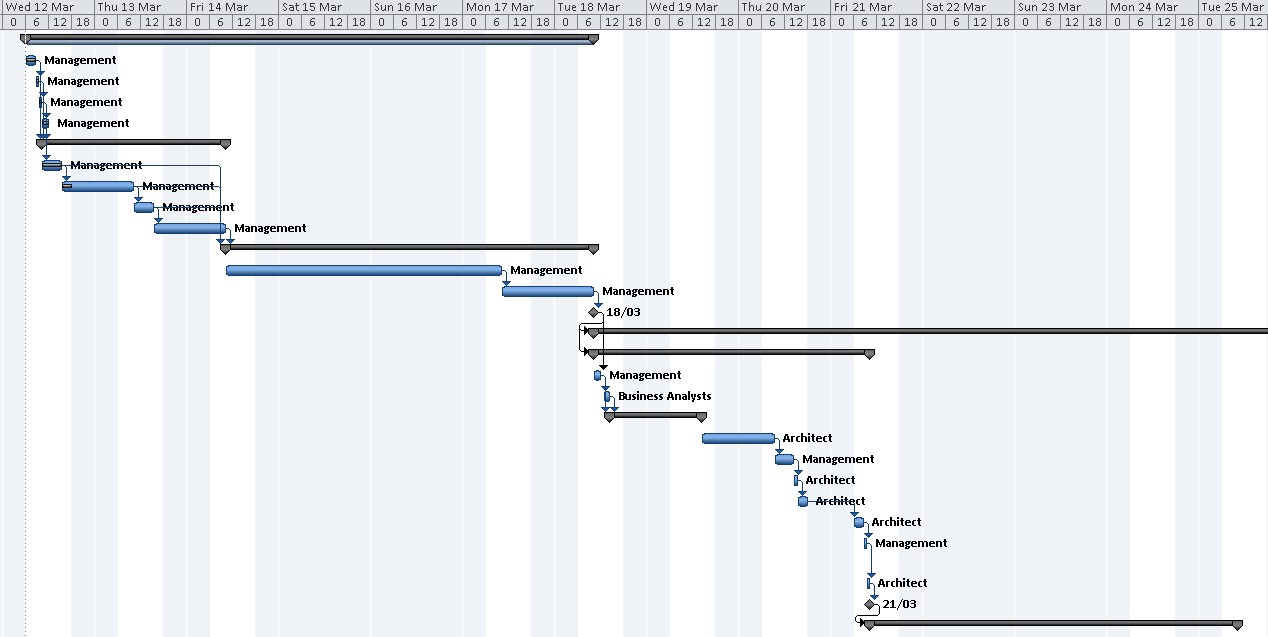
\includegraphics[width=13cm]{wbs2.png}
\end{center}
\caption{Gantt Chart }
\label{fig:letter}
\end{figure}

\section{Estimate Activities}

This is a key step in project time management where the resources for the activities and the time taken to complete these activates are done. The resources are allocated to the tasks and Work Breakdown Structures are created. The critical path is now identified and the total project duration is estimated. Expert judgement and experience from previous projects is crucial at this point.

\begin{figure} [H]
\begin{center}
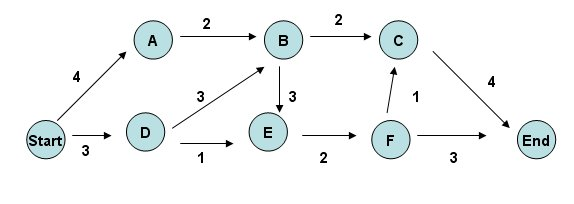
\includegraphics[scale=0.7]{ch5.png}
\caption{Critical Path}
\label{fig:criticalpath}
\end{center}
\end{figure}

\section{Develop and Control Schedule}

All information and outputs from the previous processes are now used to create a accurate schedule. Tools such as Microsoft Project are used for creating and monitoring the schedule. 

Schedule Network Analysis – This is a detailed report of how and when each stage or task should be executed. Gantt charts and network diagrams are used to graphically represent the activities and milestones which have been completed and what is left to do. 

\begin{enumerate}
\item Critical Path Method
\begin{itemize}
\item A process used to identify the critical path of a project, any delays or changes will result on your project being late.
\end{itemize}
\item Resource Levelling
\begin{itemize}
\item This process is used to identify the need for reallocation of team members in order to stay on the critical path and achieve the targeted project completion time.
\end{itemize}
\end{enumerate}

Schedule Compression is used n the event that tasks get delayed. The following two techniques are used to change the current schedule and achieve a minimum impact on the remaining project. 

\begin{enumerate}
\item Crashing 
\begin{itemize}
\item Allocating more people to complete a task or assigning team to work overtime.
\end{itemize}
\item Fast tracking
\begin{itemize}
\item Starting a task before a previous task has completed
\end{itemize}
\end{enumerate}

Schedule Control is important as if any changes to the schedule are needed, they must be re-evaluated and the project schedule must be updated.  
